\ifx\wholebook\relax \else

\documentclass[b5paper]{ctexart}
\usepackage[nomarginpar
  %, margin=.5in
]{geometry}

\addtolength{\oddsidemargin}{-0.05in}
\addtolength{\evensidemargin}{-0.05in}
\addtolength{\textwidth}{0.1in}

\usepackage[cn]{../prelude}

\setcounter{page}{1}

\begin{document}

\title{数的诞生}

\author{刘新宇
\thanks{{\bfseries 刘新宇} \newline
  Email: liuxinyu99@hotmail.com \newline}
  }

\maketitle
\fi

\markboth{数的诞生}{数的旅程}

\ifx\wholebook\relax
\chapter{数的诞生}
\numberwithin{Exercise}{chapter}
\fi

%% \epigraph{数能引导我们走向真理}{——柏拉图写给老师苏格拉底的信}

\section{数的诞生}

\begin{figure}[htbp]
 \centering
 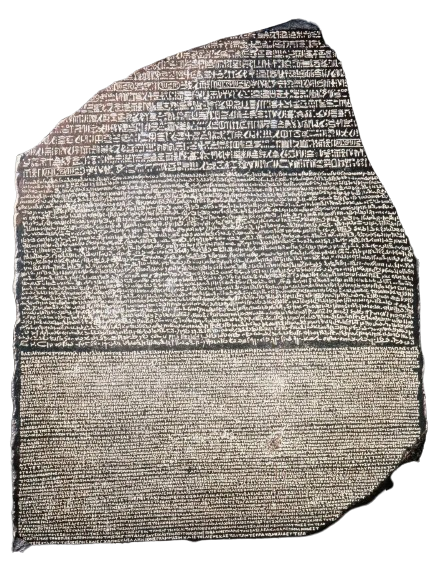
\includegraphics[scale=0.4]{img/rosetta-stone}
 \caption{罗赛塔石碑,古埃及,公元前196年}
 \label{fig:rosetta-stone}
\end{figure}


\ifx\wholebook\relax \else
\section{参考答案}
\shipoutAnswer

\begin{thebibliography}{99}

%% \bibitem{wiki-number}
%% Wikipedia. ``古代计数系统的历史''. \url{https://en.wikipedia.org/wiki/History_of_ancient_numeral_systems}

%% \bibitem{trip-to-number-kingdom}
%% [美]\ 卡尔文$\cdot$C$\cdot$克劳森\ 著\ 袁向东、袁钧\ 译. ``数学旅行家:漫游数王国''. 上海教育出版社。ISBN: 7-5320-7883-3/G $\cdot$ 7972

%% \bibitem{wiki-babylonian-num}
%% Wikipedia. ``古巴比伦数字''. \url{https://en.wikipedia.org/wiki/Babylonian_numerals}

\end{thebibliography}

\expandafter\enddocument
%\end{document}

\fi
